%************************************************
% Vergleichbare Arbeiten
%************************************************
\chapter{Vergleichbare Arbeiten}
\label{sec:related}

Es gab bereits viele Ansätze, Neulinge bei ihren ersten Schritten in der Welt der Programmierung zu unterstützen. Dazu wurden verschiedene Umgebungen und Sprachen entwickelt, die einen besonders einfachen und schnellen Einstieg -- gerade für Kinder im Schulalter -- bieten sollen. In diesem Abschnitt werden Programme hervorgehoben, die einen spielerischen Ansatz zum Lernen von Programmiersprachen bieten. Die im folgenden Abschnitt beschriebenen \nameref{sec:related:turtle}, sowie \nameref{sec:related:karel} in Abschnitt \ref{sec:related:karel}, haben als eine der ersten ihrer Art, dieses Genre maßgeblich geprägt. Während ihre Ideen ebenfalls in diese Arbeit eingeflossen sind, dient ihre Beschreibung in dieser Arbeit hauptsächlich dem historischen Kontext. \nameref{sec:related:kara} und \nameref{sec:related:lightbot} werden dabei als Vorbilder dieser Arbeit beschrieben.

%************************************************
% Turtle Grafiken
%************************************************
\section{Turtle Grafiken}
\label{sec:related:turtle}

Seymour Papert beschreibt 1980 in dem Buch \textit{Mindstorms: Children, Computers, and Powerful Ideas} seine Idee von Turtle Grafiken. Sein Ziel war die Gestaltung von Objekten, die Kinder für sich selbst und auf ihre eigene Art herstellen können. Dabei hilft ein Objekt oder eine Figur, in die sich die Kinder hineinversetzen können. Papert nennt dies das "object-to-think-with"~\cite[11]{papert1980}.

Die Schildkröte kann bewegt werden, indem Befehle über die Tastatur eingegeben werden. Die dafür entwickelte Programmiersprache heißt LOGO. \inlinec{FORWARD 100} bewegt die Schildkröte in einer geraden Linie über eine Strecke von 100 Schritten von je etwa einem Millimeter. Durch die Eingabe von \inlinec{RIGHT 90} wird die Schildkröte um 90 Grad gedreht. \inlinec{PENDOWN} lässt die Schildkröte einen Stift senken, um eine sichtbare Spur des Pfads zu hinterlassen, während \inlinec{PENUP} sie anweist, den Stift anzuheben.

Die Idee des Programmierens wird durch die Metapher eingeführt, in der der Schildkröte ein neues Wort beigebracht wird. So können \inlinec{TRIANGLE} \fref{fig:related:turtle:square:code} und \inlinec{SQUARE} \fref{fig:related:turtle:triangle:code} als Prozeduren definiert werden, die die Schildkröte ein Dreieck bzw. ein Quadrat zeichnen lassen. Diese neuen Wörter können nun verwendet werden, um Programme und neue Wörter zu definieren. Es lässt sich zum Beispiel durch Kombination eines Quadrates und eines Dreiecks ein Haus zeichnen \fref{fig:related:turtle:house:code}~\cite[12]{papert1980}.

An dieser Stelle ist zu bemerken, dass LOGO und Turtle Grafiken keine klassischen Spielmechaniken aufweisen. Der Nutzer startet immer mit einer leeren Leinwand. Für den Einsatz im Schulunterricht muss der Lehrer Aufgaben stellen, die mit den Mitteln der Sprache zu lösen sind. Eine eventuelle Ergebniskontrolle muss ebenfalls durch die Lehrkraft erfolgen.

Das im Rahmen dieser Arbeit entwickelte Programm soll eine ähnlich leicht zu verstehende Sprache verwenden, jedoch soll jede Spielwelt ein klares Ziel haben. Die Lösung einer Aufgabe kann durch den Computer überprüft werden. Dadurch wird vor allem das eigenständige Lernen gefördert und Subjektivität beim Vergleich von Lösungen der Aufgabe herausgenommen.

\begin{figure}
    \begin{subfigure}[b]{0.3\textwidth}
        \begin{lstlisting}
            TO SQUARE
            FORWARD 100
            RIGHT 90
            FORWARD 100
            RIGHT 90
            FORWARD 100
            RIGHT 90
            FORWARD 100
            RIGHT 90
            END
            \end{lstlisting}
        \caption{Code für ein Quadrat}
        \label{fig:related:turtle:square:code}
        \vspace{0.5cm}
    \end{subfigure}\hfill
    \begin{subfigure}[b]{0.3\textwidth}
        \begin{lstlisting}
            TO TRIANGLE
            FORWARD 100
            RIGHT 120
            FORWARD 100
            RIGHT 120
            FORWARD 100
            RIGHT 120
            END
            \end{lstlisting}
        \caption{Code für ein Dreieck}
        \label{fig:related:turtle:triangle:code}
        \vspace{0.5cm}
    \end{subfigure}\hfill
    \begin{subfigure}[b]{0.3\textwidth}
        \begin{lstlisting}
            TO HOUSE
            RIGHT 90
            SQUARE
            RIGHT 300
            TRIANGLE
            END
            \end{lstlisting}
        \caption{Code für ein Haus}
        \label{fig:related:turtle:house:code}
        \vspace{0.5cm}
    \end{subfigure}
    \begin{subfigure}[b]{0.3\textwidth}
        \includegraphics[width=\textwidth]{gfx/related-turtle-square.pdf}
        \caption{Ergebnis des Quadrat}
        \label{fig:related:turtle:square:result}
    \end{subfigure}\hfill
    \begin{subfigure}[b]{0.3\textwidth}
        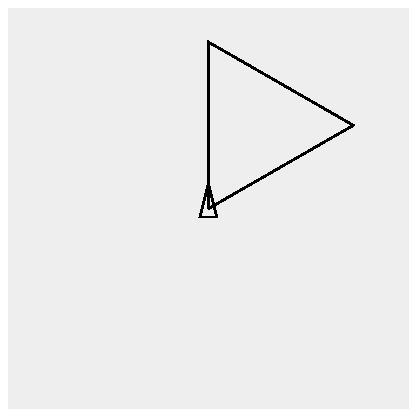
\includegraphics[width=\textwidth]{gfx/related-turtle-triangle.pdf}
        \caption{Ergebnis des Dreieck}
        \label{fig:related:turtle:triangle:result}
    \end{subfigure}\hfill
    \begin{subfigure}[b]{0.3\textwidth}
        \includegraphics[width=\textwidth]{gfx/related-turtle-house.pdf}
        \caption{Ergebnis des Haus}
        \label{fig:related:turtle:house:result}
    \end{subfigure}
    \caption{Zeichnen eines Hauses in LOGO (in Anlehnung an~\cite[14-15]{papert1980})}
    \label{fig:related:turtle:square}
\end{figure}

%************************************************
% Karel the Robot
%************************************************
\section{Karel the Robot}
\label{sec:related:karel}

Pattis geht mit \textit{Karel the Robot} einen ähnlichen Weg wie Papert mit seinen Turtle Grafiken. Aber anstelle einer Schildkröte wird der Roboter Karel über das Spielfeld bewegt. Karel bewegt sich nicht frei, sondern auf einem Netz von horizontalen (Avenue) und vertikalen Straßen (Street) auf denen sich Wände befinden können und den direkten Weg blockieren. Karel bewegt sich immer von Kreuzung zu Kreuzung. Außerdem können Gegenstände -- sogenannte Beeper -- auf Kreuzungen platziert sein. Diese können von Karel aufgenommen, bewegt und wieder abgelegt werden. Des weiteren verfügt Karel über Sensoren, die es ihm ermöglichen Wände und Gegenstände in seiner nächsten Umgebung zu detektieren. Mögliche Aufgaben beinhalten das Aufsammeln oder Ablegen von Mustern aus Gegenständen~\cite[1-3]{pattis1981}.

\begin{figure}
    \centering
    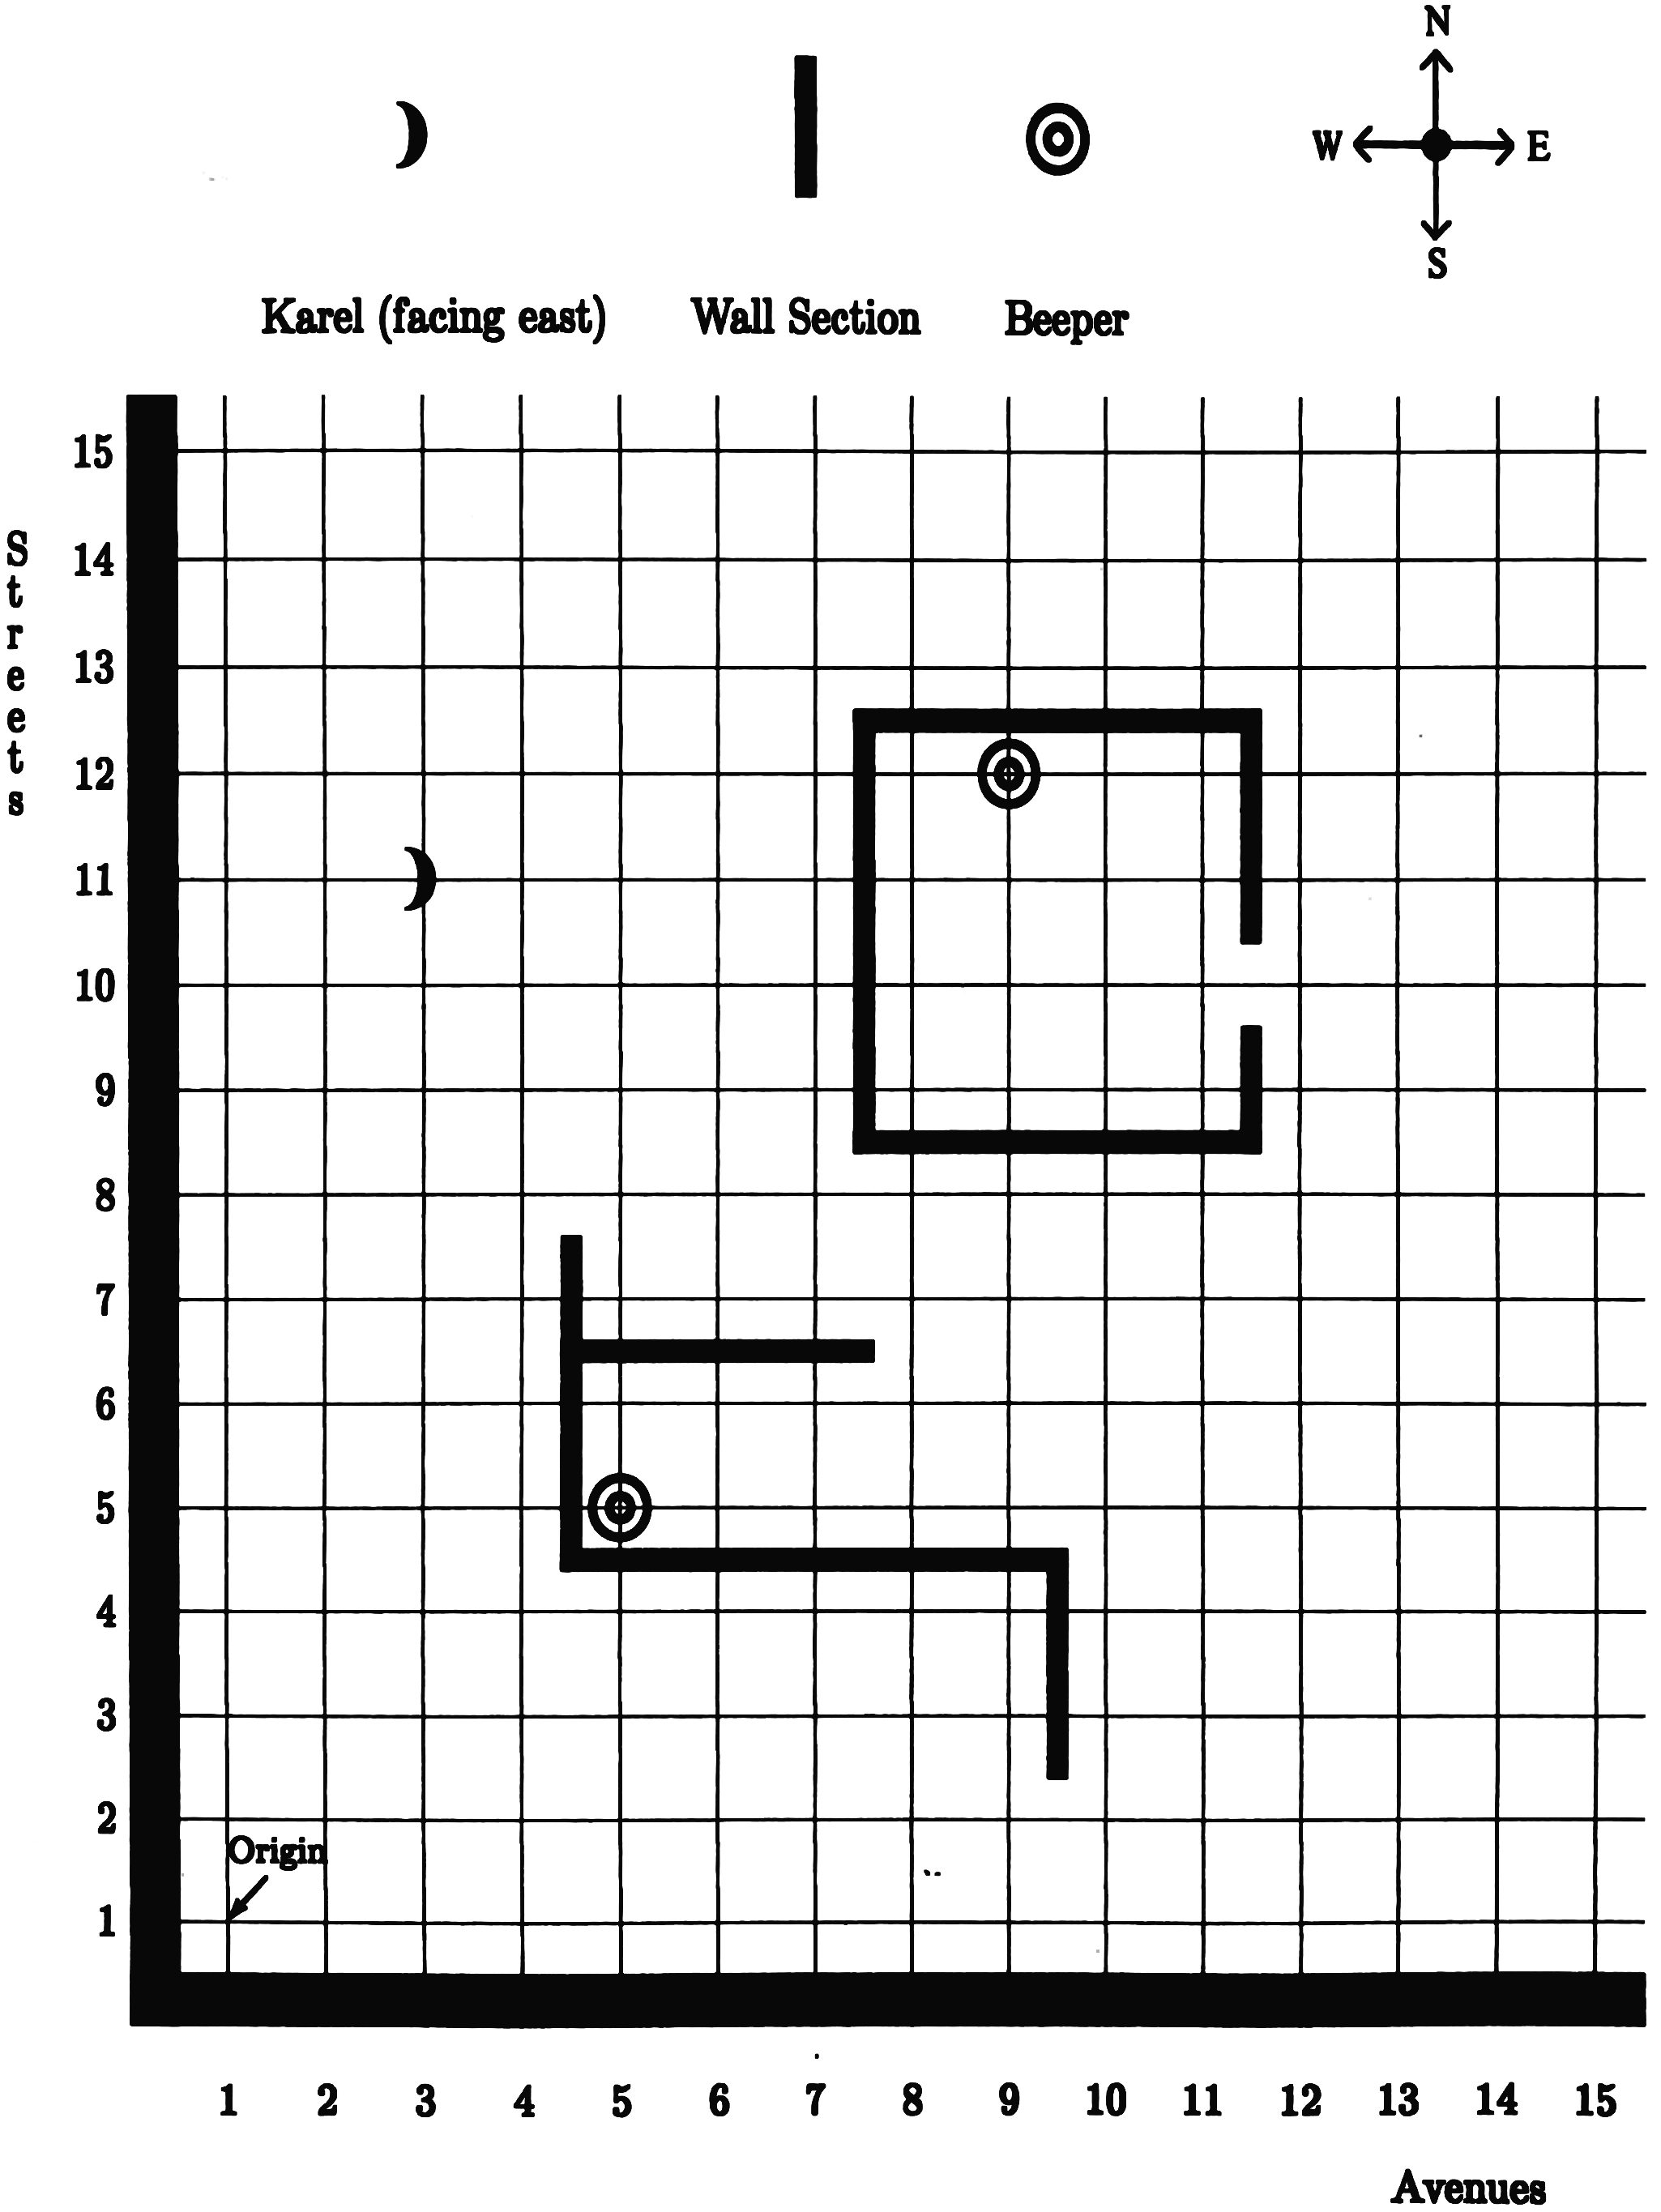
\includegraphics[width=0.5\textwidth]{gfx/related-karel.png}
    \caption{Die Struktur von Karels Welt aus~\cite[3]{pattis1981}}
    \label{fig:related:karel}
\end{figure}

Im Gegensatz zu Turtle Grafiken, startet der Nutzer bei Karel nicht mit einer leeren Seite, sondern bekommt bereits eine Welt vorgegeben, innerhalb der die Aufgabenstellung zu lösen ist. Eine mögliche Aufgabe in der in Abbildung \ref{fig:related:karel} dargestellten Welt, könnte sein: "Sammle den Beeper an Position 10/12 ein und bewege Karel zurück an seine Ausgangsposition." Eine Welt bietet also oft eine Vielzahl von Möglichkeiten für Aufgabenstellungen, allerdings müssen die Lösungen manuell kontrolliert werden.

%************************************************
% Kara
%************************************************
\section{Kara}
\label{sec:related:kara}

Kara weicht in seiner ursprünglichen Version von den vorhergenannten Programmen ab, indem auf getippte Programmierbefehle zugunsten einer grafischen Oberfläche verzichtet wird. Kara setzt hier auf das Konzept der endlichen Automaten. Reichert et al. beschreiben Kara wie folgt:

\begin{quote}
    "Kara ist eine Mini-Um\-ge\-bung basierend auf der Idee der endlichen Automaten. Kara, der Marienkäfer, lebt in einer einfachen grafischen Welt auf dem Bildschirm. Der Marienkäfer kann programmiert werden, um in seiner Welt verschiedene Aufgaben zu erledigen. Kleeblätter sammeln, einer Spur von Kleeblättern folgen oder Labyrinthe durchqueren sind einige Beispiele. Die Programme werden grafisch mit der Maus als endliche Automaten erstellt."~\cite[28]{reichert2004}
\end{quote}

Neben der ursprünglichen Idee von Kara mit endlichen Automaten, gibt es weitere Versionen, die den Übergang zu realen Programmiersprachen erleichtern sollen \cite{kara2017}. So lässt sich der Marienkäfer in der bekannten Welt auch mit Universalsprachen wie Java, JavaScript, Python oder Ruby steuern. Durch die Konstrukte, die diese Sprachen mitbringen, in Verbindung mit den speziellen Methoden, die die Kara-Um\-ge\-bung zur Verfügung stellt, sind nun auch kompliziertere Programme möglich. Abbildung \ref{fig:related:kara} zeigt eine solche Kara-Ver\-si\-on mit einem Java\-Script-Pro\-gramm, welches den vorausliegenden Baumstämmen ausweicht, bis es beim Kleeblatt am Ende angelangt und dieses entfernt. Dafür werden die von der Kara-Um\-ge\-bung bereitgestellten Sensoren zum Detektieren von Bäumen und Blättern, sowie Methoden zum Navigieren und aufgeben von Blättern eingesetzt.

Der Einsatz von Universalsprachen zur Einführung in die Programmierung bringt jedoch einige Nachteile mit sich (siehe Grundlagenkapitel \ref{sec:basics:mini-languages}) und während endliche Automaten hilfreich für ein Grundverständnis des Programmierens sein können, werden mit ihnen die Grundkonzepte des Programmierens, wie Verzweigungen, Schleifen und Funktionen, lediglich stark abstrahiert vermittelt. Für das im Rahmen dieser Arbeit entwickelte Programm soll ein Mittelweg beschritten werden, bei dem die Programmierung zwar syntaxfrei über eine grafische Oberfläche erfolgt, jedoch die Anmutung einer normalen Programmiersprache erhalten bleiben soll.

Auch bei Kara gibt es kein durch das Programm definiertes und überprüfbares Spielziel. Es kann eine Aufgabenstellung, die zu erfüllen ist, definiert und in einem seperaten Fenster angezeigt werden. Die Kontrolle obliegt allerdings dem Nutzer selbst oder dem Aufgabensteller.

\begin{figure}
    \begin{subfigure}[b]{0.5\textwidth}
        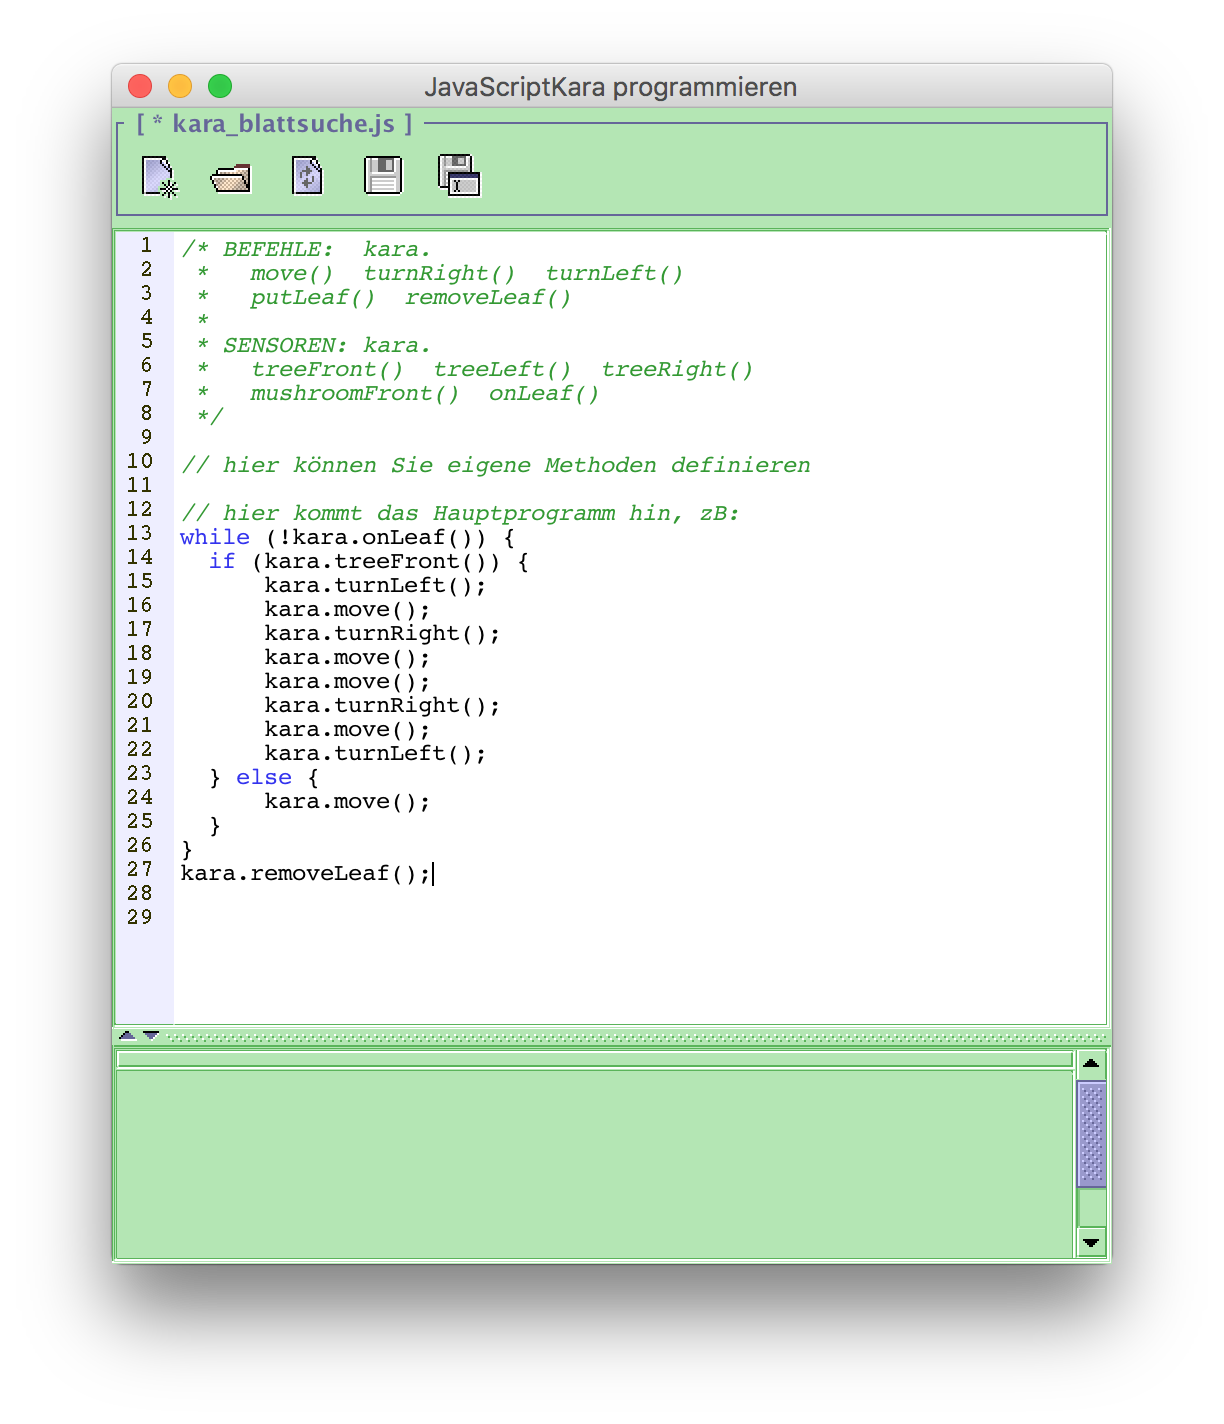
\includegraphics[width=\textwidth]{gfx/related-kara-code.png}
        \caption{Suchen eines Blattes in einem Wald}
        \label{fig:related:kara:code}
    \end{subfigure}
    \begin{subfigure}[b]{0.5\textwidth}
        \includegraphics[width=\textwidth]{gfx/related-kara-world.png}
        \caption{Kara-Welt}
        \label{fig:related:kara:world}
    \end{subfigure}
    \caption{Bildschirmfoto aus der JavaScriptKara-Anwendung}
    \label{fig:related:kara}
\end{figure}

%************************************************
% Lightbot
%************************************************
\section{Lightbot}
\label{sec:related:lightbot}

Danny Yaroslavski, der Hauptentwickler von Lightbot beschreibt sein Programm als ein Denkspiel, welches seine Mechaniken auf die Konzepte des Programmierens abbildet. Das Ziel von Lightbot ist es, in jedem Level einen Roboter dazu zu bringen, alle blauen Kacheln zu beleuchten. Dazu muss der Roboter mit einer Reihe von Anweisungen "programmiert" werden~\cite{yaroslavski2014}.

Lightbot kommt dabei gänzlich ohne geschriebene Programmieranweisungen aus. Stattdessen werden quadratische Bausteine von einer Toolbox in dafür vorgesehene Bereiche gezogen. Jeder Baustein deutet mit einem Icon den dahinterliegenden Befehl an. Prozeduren müssen verwendet werden, wenn im Bereich für das Hauptprogramm nicht ausreichend Platz vorhanden ist. Für jede Prozedur ist ein zusätzlicher Bereich vorgegeben, der mit einem entsprechenden Baustein aufgerufen werden kann.

Neben atomaren Befehlen zum Vorwärtsgehen, Links- und Rechtsdrehen, Springen und Licht an- und ausschalten, sind mit Lightbot Schleifen lediglich durch rekursive Aufrufe der Prozeduren möglich. Eine Abbruchbedingung kann nicht definiert werden. Auch auf Variablen und andere Verzweigungen wird verzichtet. Das bedeutet auch, dass der Roboter über keine Sensoren verfügt und blind durch die Spielwelt läuft. Abbildung~\ref{fig:related:lightbot:screenshot} zeigt ein Bildschirmfoto aus der Lightbot App für iOS\footnote{\url{https://itunes.apple.com/de/app/lightbot-code-hour/id873943739?mt=8}}.

Im Gegensatz zu den bisher beschriebenen Programmen, gibt es bei Lightbot ein klares Ziel, welches durch das Level definiert ist. Es müssen immer alle Lichter eingeschaltet werden. Sobald dies geschehen ist, ist das Level gelöst und das nächste Level wird freigeschaltet. Die Lösung der Aufgabenstellung muss -- im Gegensatz zu den vorgenannten Anwendungen -- nicht manuell geprüft werden und es ist mit Lightbot auch ein unbeaufsichtigtes Lernen möglich.

Die Level in der App sind in drei Gruppen aufgeteilt. Im ersten Bereich "Basics" werden die atomaren Befehle eingeführt. Dabei erhöht sich der Schwierigkeitsgrad im Laufe der 8 Level. Im zweiten Bereich "Procedures" werden dann Prozeduren eingeführt und im dritten Teil "Loops" können die Level nur durch den geschickten Einsatz von Rekursion gelöst werden.

\begin{figure}
    \centering
    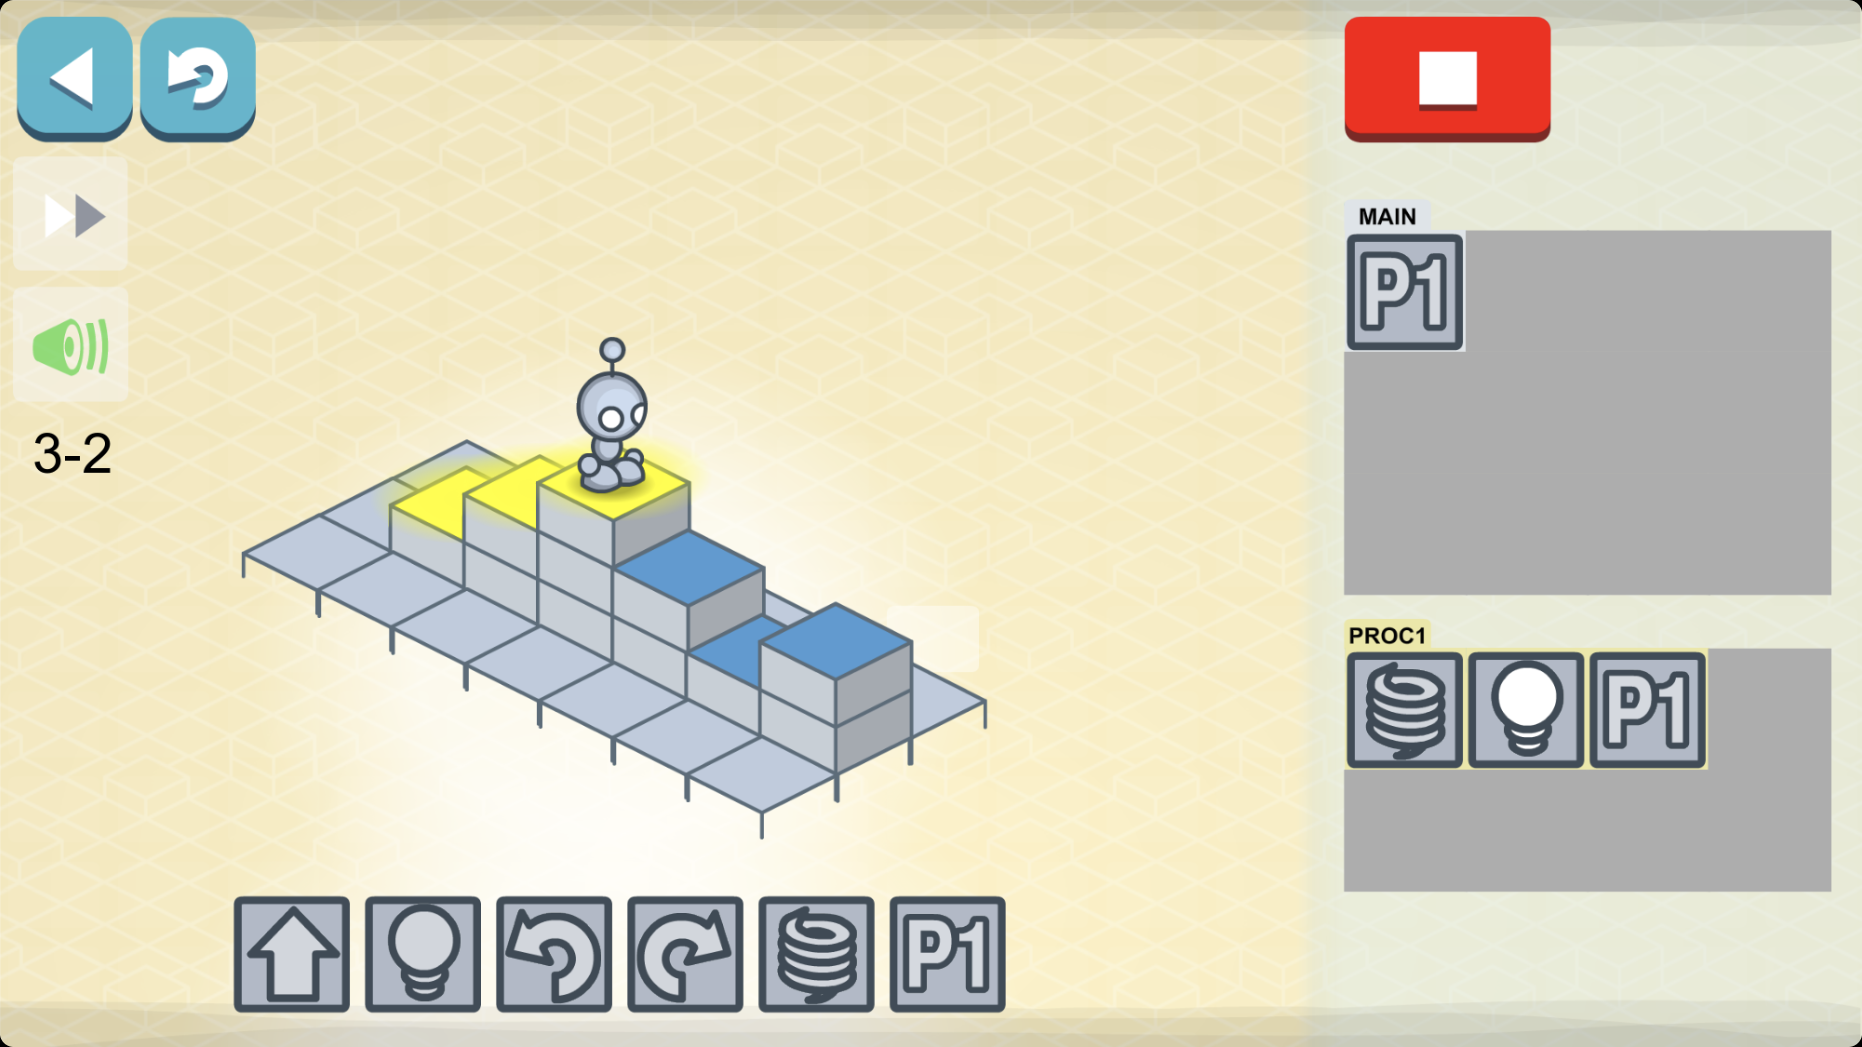
\includegraphics[width=0.8\textwidth]{gfx/related-lightbot-screenshot.png}
    \caption{Bildschirmfoto aus der Lightbot App für iOS}
    \label{fig:related:lightbot:screenshot}
\end{figure}

%************************************************
% Zusammenfassung
%************************************************
\section{Zusammenfassung}
\label{sec:related:summary}

In diesem Kapitel wurden vergleichbare Arbeiten vorgestellt, welche die Konzeption der in dieser Arbeit implementierten Umgebung maßgeblich geprägt haben. Turtle Grafiken war eine der ersten Umgebungen, in der Neulinge mit Hilfe einer Minisprache in einer Mikrowelt Programmierkonzepte erlernen können. Dabei beschränken sich diese auf das Zeichnen von Grafiken auf einer leeren Leinwand. Karel the Robot erweitert dieses Konzept um Interaktionen mit der Welt: Die Spielfigur muss durch das Spielfeld navigieren, Gegenstände einsammeln und auslegen.

Kara versucht mit endlichen Automaten einen anderen Ansatz und verzichtet auf geschriebenen Code, auch wenn die Welt und deren Interaktionsmöglichkeiten große Ähnlichkeiten zu Karel the Robot aufweisen. In weiteren Versionen ermöglicht Kara aber auch die Programmierung in anderen Programmiersprachen. Lightbot versteckt Befehle hinter Icons, die per Drag \& Drop angeordnet werden können und so ein Programm bilden.
